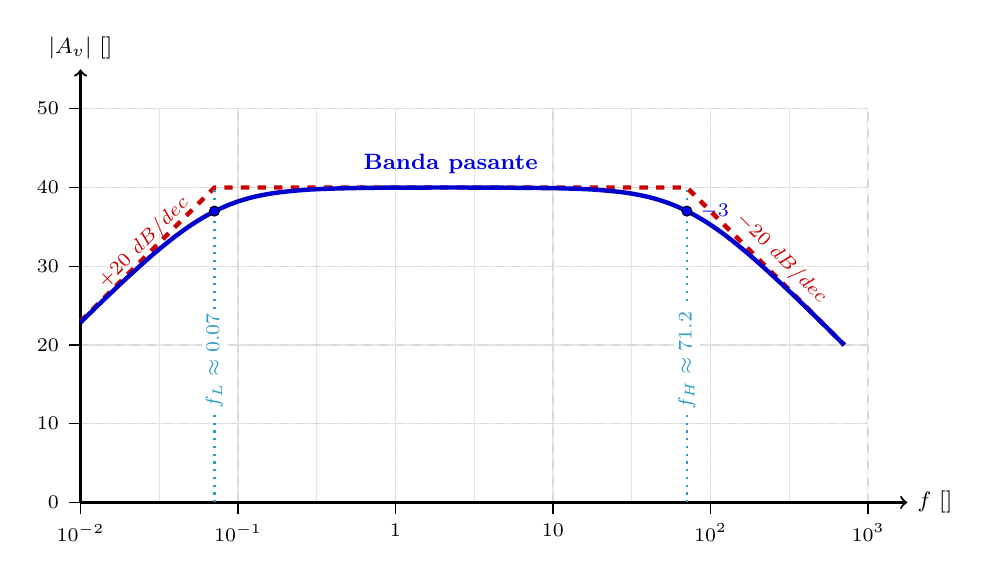
\begin{tikzpicture}[scale=1.0, transform shape]

  % Grid semilogaritmico tenue
  \draw[step=1.0, color=gray!20, thin] (0, 0) grid (10, 5);

  % Lineas de la grilla (SOLO para y > 0 y x > 0 para no superponer lineas punteadas sobre los ejes)
  \foreach \y in {1, 2, 3, 4, 5} {
    \draw[dashed, color=gray!30] (0, \y) -- (10, \y);
  }
  \foreach \x in {2, 4, 6, 8, 10} {
    \draw[dashed, color=gray!30] (\x, 0) -- (\x, 5);
  }

  % Marcas eje Y (Ganancia en dB)
  \foreach \y/\val in {0/0, 1/10, 2/20, 3/30, 4/40, 5/50} {
    \draw (0, \y) -- (-0.15, \y) node[left, font=\scriptsize] {$\val$};
  }

  % Marcas eje X (Decadas logaritmicas)
  \foreach \x/\label in {0/{$10^{-2}$}, 2/{$10^{-1}$}, 4/{$1$}, 6/{$10$}, 8/{$10^2$}, 10/{$10^3$}} {
    \draw (\x, 0) -- (\x, -0.15) node[below, font=\scriptsize] {\label};
  }

  % Ejes coordenados (dibujados solidos por encima de la grilla)
  \draw[->, thick] (0, 0) -- (10.5, 0) node[right, font=\footnotesize] {$f\ [\unit{\hertz}]$};
  \draw[->, thick] (0, 0) -- (0, 5.5) node[above, font=\footnotesize] {$|A_v|\ [\unit{\decibel}]$};

  % Curva Asintotica (linea discontinua roja)
  % fL = 0.071 Hz -> x_L = 2*(log10(0.071) + 2) = 1.70
  % fH = 71.18 Hz -> x_H = 2*(log10(71.18) + 2) = 7.70
  % Pendiente +20 dB/dec -> +1 por cada unidad de x
  \draw[dashed, ultra thick, red!80!black] 
    (0, 2.3) -- (1.70, 4.0) -- (7.70, 4.0) -- (9.70, 2.0);

  % Curva Real Suavizada (linea solida azul calculada analiticamente)
  \draw[ultra thick, blue!80!black] plot[smooth] coordinates {
    (0.00, 2.287) (0.30, 2.579) (0.60, 2.862) (0.90, 3.132) (1.20, 3.377) 
    (1.45, 3.553) (1.70, 3.697) (1.95, 3.805) (2.20, 3.880) (2.50, 3.935) 
    (2.90, 3.973) (3.40, 3.991) (4.00, 3.998) (5.00, 3.999) (6.00, 3.991) 
    (6.50, 3.974) (6.90, 3.937) (7.20, 3.882) (7.45, 3.808) (7.70, 3.701) 
    (7.95, 3.559) (8.20, 3.384) (8.50, 3.140) (8.80, 2.871) (9.10, 2.588) 
    (9.40, 2.296) (9.70, 2.000)
  };

  % Lineas de corte y singularidades con etiquetas verticales sobre las lineas
  \draw[dotted, thick, color=cyan!80!black] (1.70, 0) -- (1.70, 4.0);
  \node[fill=white, inner sep=1.5pt, font=\scriptsize, text=cyan!80!black, rotate=90] at (1.70, 1.8) {$f_L \approx \SI{0.07}{\hertz}$};

  \draw[dotted, thick, color=cyan!80!black] (7.70, 0) -- (7.70, 4.0);
  \node[fill=white, inner sep=1.5pt, font=\scriptsize, text=cyan!80!black, rotate=90] at (7.70, 1.8) {$f_H \approx \SI{71.2}{\hertz}$};

  % Anotaciones de pendientes y ganancias
  \node[above, font=\footnotesize\bfseries, color=blue!90!black] at (4.7, 4.05)
    {Banda pasante};
  \node[font=\scriptsize, color=red!80!black, rotate=45] at (0.8, 3.3) {$+20\ \text{dB/dec}$};
  \node[font=\scriptsize, color=red!80!black, rotate=-45] at (8.9, 3.1) {$-20\ \text{dB/dec}$};

  % Punto de -3dB
  \draw[fill=blue] (1.70, 3.7) circle (1.8pt);
  \draw[fill=blue] (7.70, 3.7) circle (1.8pt);
  \node[right, font=\scriptsize, color=blue!90!black] at (7.75, 3.7) {$-\SI{3}{\decibel}$};

\end{tikzpicture}
